\documentclass[11pt]{article}
\usepackage[margin=2.5cm]{geometry}
\usepackage{booktabs}
\usepackage{graphicx}
\usepackage{amsmath}
\usepackage{times}
\usepackage[hidelinks]{hyperref}
\usepackage{caption}
\captionsetup{font=small,labelfont=bf}
\usepackage{url}
\urlstyle{same}

\title{\bf Your RAG Number Is a Property of the Template You Copied:\\[2pt]
\large An Audit of the Default Question-Answering Prompts Shipped by Three RAG Frameworks}

\author{Fangqi Liu\textsuperscript{1,*}\quad Yuhe Liu\textsuperscript{1}\\[4pt]
\small \textsuperscript{1}\textit{Affiliation to be completed}\\
\small \textsuperscript{*}\textbf{Corresponding author:} Fangqi Liu\\ \small \texttt{fangqiliu404@gmail.com}}

\date{}

\begin{document}
\maketitle

\begin{abstract}
\noindent
Retrieval-augmented generation (RAG) systems are usually built by copying a default
question-answering prompt from a framework, yet the choice among those defaults is almost
never reported. We take the default prompts shipped by three widely used frameworks ---
LangChain, LlamaIndex and FlashRAG --- verbatim, and run all three on the same readers, the
same documents and the same three multi-hop QA datasets. Measured exact match differs by up
to \textbf{46 points} (HotpotQA: 46.4 for FlashRAG, 0.0 for the other two), while a
format-insensitive measure --- whether the gold answer appears anywhere in the response ---
differs by under five points and is not significant (McNemar $p=0.54$). The gap is produced
by response style: 19 versus 134 characters. A second, independent effect comes from one
sentence inside LangChain's default, which instructs the reader to say that it does not know.
With an empty context that sentence drives abstention to \textbf{79--95\%}, against
\textbf{0--2\%} once it is deleted and nothing else changed; the deletion also removes 6--8
points of the apparent benefit of retrieval. The effect is not monotone in model size: a
Llama-3.2-1B reader abstains on \textbf{91.5\%} of questions \emph{with the documents
present} under that template and 0.0\% under LlamaIndex's ($p=1.6\times10^{-55}$). The
closed-book half of our comparison is anchored against FlashRAG's published setting
(HotpotQA F1 24.9 against a reported 28.4). We recommend that RAG evaluations report the
template verbatim, the answer format, and abstention separately from accuracy.

\vspace{4pt}
\noindent\textbf{Keywords:} retrieval-augmented generation; evaluation methodology; prompt
templates; answer extraction; abstention; reproducibility

\end{abstract}

\section{Introduction}

A retrieval-augmented generation system is assembled from components: a retriever, a reranker,
a reader, and a prompt that glues them together~\cite{lewis2020rag,gao2023survey}. The first
three are usually described in detail. The prompt is usually a line of code copied from a
framework's default, and its exact wording is rarely reported.

This paper asks a narrow, practical question: if three practitioners build the same RAG
pipeline on the same reader and the same documents, but each copies a different framework's
default prompt, how far apart will their reported numbers be?

The answer, on HotpotQA~\cite{yang2018hotpotqa} with a Qwen2.5-3B reader, is
\textbf{46 exact-match points}: 46.4 for the FlashRAG template, and exactly 0.0 for the
LangChain and LlamaIndex templates. The readers are identical, the documents identical, the questions identical.

The gap does not come from knowledge. A format-insensitive measure --- does the gold string
appear anywhere in the response --- puts the three templates within five points of each other,
with no significant difference between the two extremes. The models produce the same content;
one template asks for a short span and gets one, the other two ask for an explanation and get
134 characters instead of 19. Under exact match, the second kind of response scores zero even
when the answer is inside it.

A second effect runs in the opposite direction and is not a measurement artefact at all.
LangChain's default contains the sentence \emph{``If you don't know the answer, just say that
you don't know, don't try to make up an answer.''} With an empty context, that sentence drives
the reader to refuse on 79--95\% of questions. Deleting that sentence and nothing else drops
abstention to 0--2\%, while the format-insensitive measure barely moves: the sentence changes
whether the reader speaks, not what it would have said. The practical consequence is that the
``closed-book baseline'' reported in many RAG papers measures a refusal policy installed by
the template, and that it inflates the measured benefit of retrieval by six to eight points in
our data.

The two effects belong to different classes. The first is an evaluation artefact of the kind
analysed by Sclar et al.~\cite{sclar2024quantifying}, Voronov et
al.~\cite{voronov2024mind}, Mizrahi et al.~\cite{mizrahi2024state} and Hua et
al.~\cite{hua2025flaw}: the model knows the answer, the metric cannot see it. The second is a
behavioural change: the model abstains because it was told to. Reporting the number without
distinguishing them is what makes RAG results hard to compare.

\subsection*{Contributions}
\begin{enumerate}
\item We take three published default templates verbatim, with provenance, and measure what a
practitioner copying each would report: a 46-point exact-match spread on identical inputs
(Section~\ref{sec:format}).
\item We show the spread is response style rather than knowledge, using a containment measure
and a truncation probe that rules out the ``short answer buried in prose'' explanation
(Section~\ref{sec:mechanism}).
\item We isolate one sentence of one template with a byte-level ablation and three control
variants, and show it controls the closed-book baseline (Section~\ref{sec:clause}).
\item We characterise reader dependence across two model families and four sizes, and find
that compliance is a property of the family as much as of the size
(Section~\ref{sec:readers}).
\item We anchor the closed-book half of the comparison against a published evaluation setting
(Section~\ref{sec:anchor}).
\end{enumerate}

We claim no new method. Every component is standard: BM25 retrieval, greedy decoding, exact
match and token F1. The contribution is an audit of defaults, and it stands or falls on
whether the measured spread reproduces --- which is why every number in this paper is
regenerated from raw prediction files by a script.

\section{Related work}

\paragraph{Prompt and format sensitivity.}
Sclar et al.~\cite{sclar2024quantifying} show that spurious features of prompt formatting can
move benchmark accuracy by tens of points, and introduce a spread metric to quantify it.
Voronov et al.~\cite{voronov2024mind} make the same point for in-context learning comparisons,
and Mizrahi et al.~\cite{mizrahi2024state} argue for multi-prompt evaluation as a default.
Webson and Pavlick~\cite{webson2022prompt} examine whether models actually use prompt meaning
or surface form. Our Section~\ref{sec:format} is a concrete instance of this literature,
measured on a different object: not templates the authors wrote, but the three defaults that
frameworks ship, which is what a practitioner actually copies.

\paragraph{Evaluation as an artefact source.}
Hua et al.~\cite{hua2025flaw} show that much of the reported prompt sensitivity originates in
heuristic evaluation, in particular rigid answer matching, and that it shrinks under
LLM-as-a-judge~\cite{zheng2023judging} scoring. Our result is the same mechanism with a
measured magnitude on shipped defaults. Broader work on reproducible
evaluation~\cite{liang2023helm,biderman2024lessons} makes the complementary point that
harness-level choices dominate many reported differences.

\paragraph{Abstention and calibration.}
A line of work documents that a model's willingness to abstain is largely installed by the
prompt rather than by its knowledge~\cite{abstention2025}, and that models can estimate their
own uncertainty when asked in the right
way~\cite{kadavath2022language,kuhn2023semantic,farquhar2024detecting}. We extend the
instructional account from the retrieval condition to the \emph{closed-book baseline}: the
template most practitioners copy makes that baseline near-silent.

\paragraph{RAG systems and toolkits.}
Retrieval-augmented generation spans dense retrieval~\cite{karpukhin2020dense},
fusion-in-decoder readers~\cite{izacard2021leveraging}, and adaptive or self-reflective
variants~\cite{asai2024selfrag,jiang2023flare}. FlashRAG~\cite{flashrag2025} documents its
evaluation setting explicitly --- Llama3-8B-instruct, e5-base-v2, five documents --- and
reports HotpotQA F1 of 35.3 for standard RAG and 28.4 without retrieval; we use those as the
anchor in Section~\ref{sec:anchor}. LangChain~\cite{langchain} and LlamaIndex~\cite{llamaindex}
ship the templates of Section~\ref{sec:templates} as their default retrieval-QA prompts. None
of these projects is at fault for the numbers; the point is that the choice among them is
unmade and unstated in most downstream work.

\paragraph{Benchmarks.}
We use HotpotQA (distractor setting)~\cite{yang2018hotpotqa}, 2WikiMultiHopQA~\cite{ho2020},
and MuSiQue~\cite{trivedi2022musique}, with exact match and token F1, the metrics established
by extractive QA benchmarks~\cite{rajpurkar2016squad}, and follow the multi-hop evaluation
conventions of Bamboogle~\cite{press2023measuring}.

\section{The three published defaults}
\label{sec:templates}

We did not write a prompt. Table~\ref{tab:templates} lists the three templates, reproduced
verbatim from their sources, with the sentence that matters and the output cue that shapes the
response.

\begin{table}[t]
\centering
\caption{The three default QA templates, verbatim, with provenance.}
\label{tab:templates}
\small
\begin{tabular}{@{}p{1.2cm}p{7.0cm}p{1.6cm}p{2.6cm}@{}}
\toprule
id & source & abstention clause & output cue \\
\midrule
LC & \texttt{langchain.chains} \texttt{retrieval\_qa.prompt} & \textbf{yes} & \texttt{Helpful Answer:} \\
LI & \texttt{llama\_index} \texttt{DEFAULT\_TEXT\_QA\_PROMPT} & no & \texttt{Answer:} \\
FR & FlashRAG \texttt{base\_prompt} (answer prompt) & no & \texttt{Answer:} \\
\bottomrule
\end{tabular}
\end{table}

The LangChain template reads, verbatim:

\begin{quote}\small
Use the following pieces of context to answer the question at the end. If you don't know the
answer, just say that you don't know, don't try to make up an answer.\\
\{context\}\\
Question: \{question\}\\
Helpful Answer:
\end{quote}

The abstention sentence is the second sentence; the output cue is the last line. Both will
matter, for different reasons.

\section{Experimental setup}

\paragraph{Readers.} Four instruction-tuned models served locally through a quantised runtime
at 4 bits: Llama-3.2-1B, Qwen2.5-3B (primary), Qwen2.5-7B, and Llama3-8B. Decoding is greedy
with a fixed seed and a generation cap of 32 tokens. The model families are those of
Qwen~\cite{qwen2024} and Llama 3~\cite{llama3}.

\paragraph{Data.} HotpotQA (distractor), 2WikiMultiHopQA, and MuSiQue held-out slices, 500
questions each, with a frozen question list. Each question is accompanied by its ten candidate
paragraphs; we order them by BM25 and present all ten.

\paragraph{Conditions.} \emph{rag}: the ten documents are inserted into the template.
\emph{closed}: the context slot is empty and nothing else changes.

\paragraph{Clause ablation.} Four variants of LC differing only in that sentence:
\texttt{LC} unchanged (209 characters), \texttt{LC\_minus} sentence deleted (117),
\texttt{LC\_cleared} replaced by the empty string (118), and \texttt{LC\_neutral} replaced by an
equal-length neutral sentence (217). Four variants, one variable.

\paragraph{Metrics.} Exact match (EM) after standard normalisation; token F1;
\emph{containment} (does the gold answer appear anywhere in the response, case-insensitive);
and \emph{abstention} (the response is empty or is a refusal). Containment is reported because
those templates elicit prose, for which EM is uninformative by construction.

\paragraph{Scale.} 21{,}000 reader calls in total. All predictions are stored per question and
every number in the paper is regenerated from them by a single verification script, which
recomputes 40 quoted values and compares them with the manuscript.

\section{Results}

\subsection{The template decides whether EM is measurable}
\label{sec:format}

Table~\ref{tab:format} reports the retrieval condition with the Qwen2.5-3B reader.

\begin{table}[t]
\centering
\caption{Retrieval condition, Qwen2.5-3B, $n=500$ per cell. Containment is within five points
across templates while EM spans 12--46 points.}
\label{tab:format}
\begin{tabular}{@{}llrrrr@{}}
\toprule
dataset & template & EM & F1 & containment & abstention \\
\midrule
HotpotQA & FR & \textbf{46.4} & 58.2 & 50.6 & 0.0 \\
         & LI & 0.0 & 12.3 & 47.8 & 0.0 \\
         & LC & 0.0 & 13.3 & 52.2 & 0.8 \\
\midrule
2Wiki    & FR & \textbf{37.8} & 44.4 & 44.4 & 0.2 \\
         & LI & 0.0 & 10.2 & 40.4 & 0.2 \\
         & LC & 0.0 & 11.8 & 43.0 & 6.2 \\
\midrule
MuSiQue  & FR & \textbf{12.2} & 19.9 & 15.2 & 1.0 \\
         & LI & 0.0 & 4.5 & 10.4 & 0.0 \\
         & LC & 0.0 & 4.5 & 10.2 & 6.0 \\
\bottomrule
\end{tabular}
\end{table}

On HotpotQA the FlashRAG template reaches 46.4 EM and the other two exactly 0.0, a difference
of 46 points on identical inputs. Containment, however, is 50.6, 47.8 and 52.2; the paired
difference between FlashRAG and LangChain is $-1.6$ with an exact McNemar
$p=0.54$, and between LlamaIndex and LangChain $-4.4$ with $p=0.008$.

The same pattern holds on the other two datasets: EM spreads by 12--38 points while
containment stays within five. Figure~\ref{fig:em} repeats the comparison across all four
readers; in every case the FlashRAG template is far above the other two.

\begin{figure}[t]
\centering
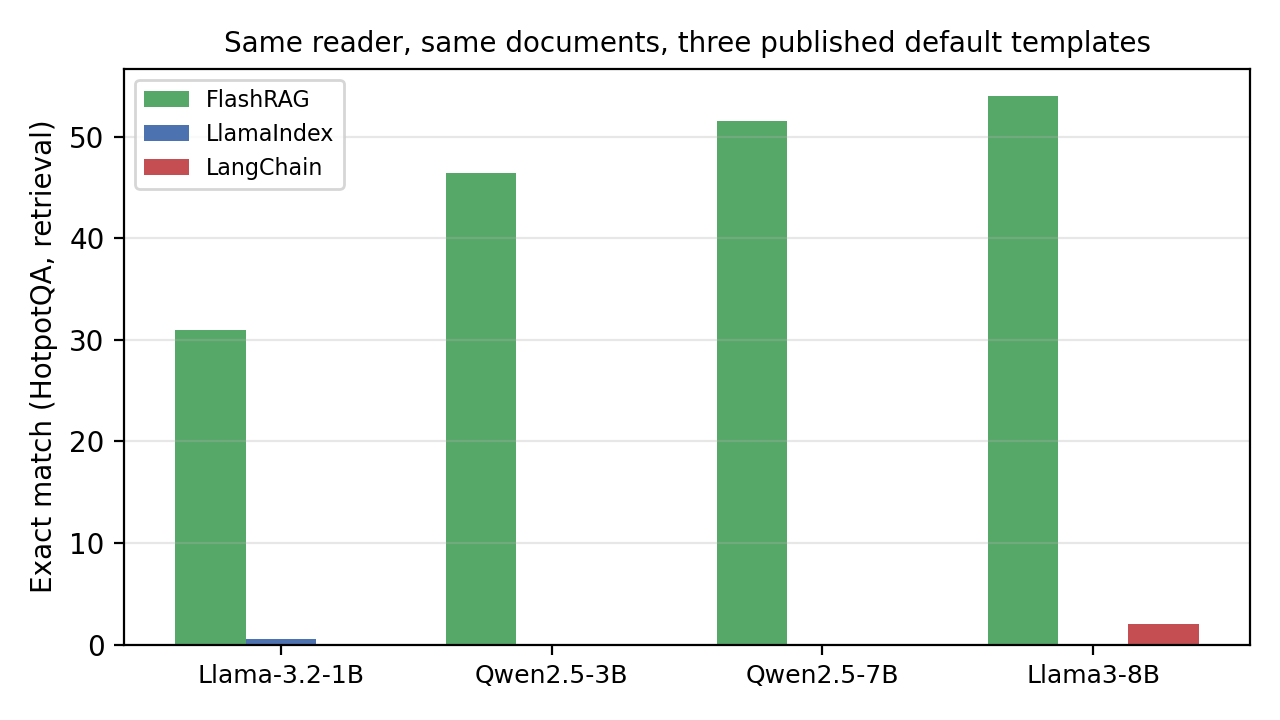
\includegraphics[width=0.78\linewidth]{fig_templates.png}
\caption{Exact match on HotpotQA (retrieval condition) for the same reader, the same
documents and the same questions, under three published default templates.}
\label{fig:em}
\end{figure}

A practitioner who copies LangChain's default would conclude, from any of these three
datasets, that the reader cannot answer the question at all.

\subsection{Mechanism: response style, not knowledge}
\label{sec:mechanism}

Table~\ref{tab:length} reports mean response length. The FlashRAG template yields 19-character
answers; the other two yield 133--141.

\begin{table}[t]
\centering
\caption{Response length, HotpotQA, retrieval condition. The seven-fold difference in length
is the whole of the EM gap.}
\label{tab:length}
\begin{tabular}{@{}lrrrr@{}}
\toprule
template & mean chars & median chars & EM & containment \\
\midrule
FR & \textbf{19} & 12 & 46.4 & 50.6 \\
LI & 134 & 136 & 0.0 & 47.8 \\
LC & 133 & 134 & 0.0 & 52.2 \\
LC\_minus & 139 & 140 & 0.0 & 48.4 \\
LC\_neutral & 141 & 142 & 0.0 & 45.4 \\
\bottomrule
\end{tabular}
\end{table}

One might assume that a short answer is buried at the front of the prose and simply needs to be
extracted. It is not. Truncating every response to its first $w$ words and re-scoring gives
Table~\ref{tab:trunc}.

\begin{table}[t]
\centering
\caption{Exact match after truncating the response to its first $w$ words.}
\label{tab:trunc}
\begin{tabular}{@{}lrrrrr@{}}
\toprule
template & full & $w=3$ & $w=5$ & $w=8$ & $w=15$ \\
\midrule
FR & 46.4 & 41.8 & 45.8 & 46.6 & 46.6 \\
LI & 0.0 & 1.4 & 0.2 & 0.0 & 0.0 \\
LC & 0.0 & 1.2 & 0.2 & 0.0 & 0.0 \\
LC\_minus & 0.0 & 0.8 & 0.2 & 0.0 & 0.0 \\
\bottomrule
\end{tabular}
\end{table}

Truncation recovers at most 1.4 points. The correct string is present somewhere in about half
of the LangChain responses (containment 52.2), but the model never leads with it: the template
shifts the task from extraction to commentary. Under a strict-match metric, a commentary is
worth zero.

\subsection{The clause decides what the closed-book baseline measures}
\label{sec:clause}

LangChain's default contains one sentence that no other template in our set contains. With an
empty context, that sentence dominates the behaviour (Table~\ref{tab:clause}).

\begin{table}[t]
\centering
\caption{Abstention rate with an empty context, Qwen2.5-3B, $n=500$. The clause is the whole
difference.}
\label{tab:clause}
\begin{tabular}{@{}lrrrr@{}}
\toprule
dataset & LC & LC\_minus & LC\_neutral & LC\_cleared \\
\midrule
HotpotQA & \textbf{91.2} & 1.0 & 0.2 & 1.4 \\
2Wiki    & \textbf{79.0} & 0.0 & 0.2 & 0.0 \\
MuSiQue  & \textbf{95.0} & 2.0 & 0.0 & 1.6 \\
\bottomrule
\end{tabular}
\end{table}

Deleting that one sentence --- leaving the template byte-identical otherwise --- moves
abstention from 79--95\% to 0--2\%. The equal-length neutral replacement reproduces the
collapse, so the effect is the sentence's content and not its length.

Critically, containment in the same condition barely moves: 11.2 under LC and 14.4 under
LC\_minus on HotpotQA (28.6 and 31.8 on 2Wiki). The sentence does not change what the reader
would say; it changes whether the reader says anything.

The consequence for a standard comparison is in Table~\ref{tab:gap}: the clause inflates the
apparent benefit of retrieval by 8.2 points on HotpotQA and 6.0 on 2Wiki.

\begin{table}[t]
\centering
\caption{Retrieval minus closed book, in containment points. The clause inflates the apparent
benefit of retrieval.}
\label{tab:gap}
\begin{tabular}{@{}lrrrr@{}}
\toprule
dataset & LC & LC\_minus & LC\_neutral & LC\_cleared \\
\midrule
HotpotQA & 41.0 & 34.0 & 34.2 & 32.8 \\
2Wiki    & 14.4 & 8.4 & 8.2 & 11.8 \\
MuSiQue  & 10.2 & 9.2 & 8.6 & 11.0 \\
\bottomrule
\end{tabular}
\end{table}

\subsection{Reader dependence}
\label{sec:readers}

We repeated the comparison for four readers. Table~\ref{tab:readers} shows that the two effects
behave differently.

\begin{table}[t]
\centering
\caption{HotpotQA, retrieval condition unless stated, $n=200$ per cell.}
\label{tab:readers}
\begin{tabular}{@{}llrrr@{}}
\toprule
reader & template & EM & containment & abstention \\
\midrule
Llama3-8B & FR & \textbf{54.0} & 56.5 & 0.0 \\
          & LC & 2.0 & 45.5 & \textbf{22.0} \\
          & LI & 0.0 & 42.5 & 0.0 \\
          & LC (closed) & 0.0 & 6.0 & \textbf{80.0} \\
\midrule
Qwen2.5-7B & FR & 51.5 & 57.5 & 0.0 \\
           & LC & 0.0 & 52.5 & 0.0 \\
           & LC (closed) & 0.0 & 17.0 & 15.0 \\
\midrule
Qwen2.5-3B & FR & 46.4 & 50.6 & 0.0 \\
           & LC & 0.0 & 52.2 & 0.8 \\
           & LC (closed) & 0.0 & 11.2 & \textbf{91.2} \\
\midrule
Llama-3.2-1B & FR & 31.0 & 33.0 & 0.0 \\
             & LC & 0.0 & \textbf{6.5} & \textbf{91.5} \\
             & LI & 0.5 & 44.5 & 0.0 \\
\bottomrule
\end{tabular}
\end{table}

\emph{The format effect is universal.} At every reader, the prose-eliciting templates collapse
to zero or near-zero EM while FlashRAG's reaches 31--54.

\emph{Compliance varies by family as much as by size.} Qwen2.5-7B abstains on 0.0\% of questions
with documents present; Llama3-8B, on the same template and data, abstains on 22.0\%. A 7B
model from one family resists an instruction that an 8B model from another obeys.

\emph{The smallest reader is the most compliant.} Llama-3.2-1B answers 91.5\% of the time with
\emph{no} documents, and refuses 91.5\% of the time when the documents are right there under
LangChain's template. The paired comparison against LlamaIndex's template is decisive: 91.5\%
versus 0.0\% abstention, exact McNemar $p=1.6\times10^{-55}$ with 183 discordant pairs, all in
one direction, and containment 6.5 versus 44.5.

\subsection{Anchor against a published setting}
\label{sec:anchor}

An audit is only useful if its instrument is calibrated. FlashRAG publishes its reader
configuration --- Llama3-8B-instruct, e5-base-v2, five documents --- together with HotpotQA F1
of 35.3 for standard RAG and 28.4 without retrieval. Table~\ref{tab:anchor} compares our run of
that reader under that template.

\begin{table}[t]
\centering
\caption{Anchor. The closed-book condition, which has no retriever, agrees to within 3.5 F1.}
\label{tab:anchor}
\begin{tabular}{@{}llrr@{}}
\toprule
condition & retriever & ours (F1) & FlashRAG reported (F1) \\
\midrule
closed book & none & \textbf{24.9} & \textbf{28.4} \\
retrieval & ours: 10-doc pool & 67.6 & 35.3 (e5, 1M corpus) \\
\bottomrule
\end{tabular}
\end{table}

The closed-book condition agrees to within 3.5 points, and it is the condition in which there
is no retriever, hence nothing else that could differ. That is our calibration point: the
reader, the prompt and the metric behave like the published pipeline.

The retrieval condition does not agree, and the reason is known: their retriever scores five
paragraphs from a one-million-document Wikipedia corpus, whereas our pool contains the gold
paragraph by construction. In a separate experiment in our project, open-corpus retrieval
placed the full gold paragraph set in the top ten for only 59\% of questions, against 100\% for
the pool. That gap, not the reader, accounts for the difference.

\section{Discussion}

Taken together, the two effects say something simple: \emph{the reported number is a property
of the template, and the template is rarely reported.}

The format effect is an evaluation artefact in the sense of Hua et al.~\cite{hua2025flaw}: the
knowledge is there, the metric cannot see it. It is nevertheless an artefact that produces a
46-point difference between two systems that are, in every other respect, identical, and it is
not hypothetical --- it is the difference between the defaults that two of the most widely used
frameworks ship.

The clause effect is not an evaluation artefact at all: removing it changes behaviour, not
scoring. It matters because the closed-book condition is the standard evidence that ``retrieval
helps'', and in the default configuration that condition is largely measuring a refusal policy.
The inflation we measure, 6--8 points, is of the same order as the differences RAG papers
routinely claim.

\paragraph{Recommendations.}
\begin{enumerate}
\item Report the template verbatim. ``We use a standard RAG prompt'' spans a 46-point range.
\item Report abstention separately from accuracy. The identity $\mathrm{EM}=(1-u)\,c$, with
$u$ the abstention rate and $c$ the conditional accuracy, makes the policy term explicit.
\item If exact match is the metric, use a short-answer cue; otherwise report F1 or containment,
because prose responses score zero by construction.
\item When claiming an instruction effect, include a neutral-sentence control: our equal-length
replacement reproduces the abstention collapse, which rules out length.
\end{enumerate}

\section{Threats to validity}

\emph{Scale.} Two model families and four sizes, all quantised to 4 bits, on one machine. The
absolute levels are specific to these readers.

\emph{Retriever.} One sparse retriever over a per-question pool. The retrieval condition is
therefore not comparable with open-corpus results, as Section~\ref{sec:anchor} shows
explicitly. All our claims are within-stack comparisons.

\emph{Templates.} Three templates is a sample, not a census; other frameworks may ship other
defaults. The clause ablation exists only for LangChain, because the other two templates have
no abstention sentence to delete --- which is itself part of the finding.

\emph{Generality.} We test English multi-hop QA. Whether the same spread appears in
single-hop QA, in other languages, or with API-based readers is untested.

\section{Conclusion}

Three frameworks ship three different default prompts, and on the same reader and the same
documents those prompts produce exact matches of 46.4, 0.0 and 0.0, while a format-insensitive
measure puts them within five points of one another. One sentence inside one of those defaults
additionally drives the closed-book baseline to near silence, and inflates the apparent benefit
of retrieval by six to eight points. Neither effect is exotic; both follow from defaults that
are copied without being read. Reporting the template, the answer format and the abstention
rate costs three lines and makes the number interpretable.

\section*{Declarations}

\noindent\textbf{Funding.} Not applicable.

\noindent\textbf{Competing interests.} The authors declare no competing interests.

\noindent\textbf{Ethics approval.} Not applicable; the study uses public benchmarks and locally
served open-weight models.

\noindent\textbf{Consent to participate / for publication.} Not applicable.

\noindent\textbf{Data availability.} All datasets are public
(HotpotQA~\cite{yang2018hotpotqa}, 2WikiMultiHopQA~\cite{ho2020}, MuSiQue~\cite{trivedi2022musique}).
Per-question predictions and the scripts that regenerate every table are available in the
project repository; see Code availability.

\noindent\textbf{Code availability.} The runner that produces the predictions, the analysis
scripts, the figure scripts, and the verification script that recomputes all 40 quoted values
are released at \url{https://github.com/910244720/rag-template-audit} (to be made public upon
acceptance).

\noindent\textbf{Author contributions.} Fangqi Liu: conceptualisation, methodology, software,
investigation, formal analysis, writing --- original draft. Yuhe Liu: data curation,
validation, writing --- review and editing. Both authors read and approved the final
manuscript.

\begin{thebibliography}{99}

\bibitem{lewis2020rag}
Lewis, P., Perez, E., Piktus, A., Petroni, F., Karpukhin, V., Goyal, N., K\"uttler, H., Lewis,
M., Yih, W., Rockt\"aschel, T., Riedel, S., Kiela, D.: Retrieval-augmented generation for
knowledge-intensive NLP tasks. In: Advances in Neural Information Processing Systems (NeurIPS)
(2020)

\bibitem{karpukhin2020dense}
Karpukhin, V., O\u{g}uz, B., Min, S., Lewis, P., Wu, L., Edunov, S., Chen, D., Yih, W.: Dense
passage retrieval for open-domain question answering. In: Proceedings of EMNLP (2020)

\bibitem{izacard2021leveraging}
Izacard, G., Grave, E.: Leveraging passage retrieval with generative models for open domain
question answering. In: Proceedings of EACL (2021)

\bibitem{gao2023survey}
Gao, Y., Xiong, Y., Gao, X., Jia, K., Pan, J., Bi, Y., Dai, Y., Sun, J., Wang, H.: Retrieval-
augmented generation for large language models: a survey.
\url{https://arxiv.org/abs/2312.10997} (2023)

\bibitem{asai2024selfrag}
Asai, A., Wu, Z., Wang, Y., Sil, A., Hajishirzi, H.: Self-RAG: learning to retrieve, generate,
and critique through self-reflection. In: International Conference on Learning
Representations (ICLR) (2024)

\bibitem{jiang2023flare}
Jiang, Z., Xu, F., Gao, L., Sun, Z., Liu, Q., Dwivedi-Yu, J., Yang, Y., Callan, J.,
Neubig, G.: Active retrieval augmented generation. In: Proceedings of EMNLP (2023)

\bibitem{sclar2024quantifying}
Sclar, M., Choi, Y., Tsvetkov, Y., Suhr, A.: Quantifying language models' sensitivity to
spurious features in prompt design, or: how I learned to start worrying about prompt
formatting. In: International Conference on Learning Representations (ICLR) (2024)

\bibitem{voronov2024mind}
Voronov, A., Wolf, L., Ryabinin, M.: Mind your format: towards consistent evaluation of
in-context learning improvements. \url{https://arxiv.org/abs/2401.06766} (2024)

\bibitem{mizrahi2024state}
Mizrahi, M., Kaplan, G., Malkin, D., Dror, R., Shahaf, G., Stanovsky, G.: State of what art? A
call for multi-prompt LLM evaluation. Transactions of the Association for Computational
Linguistics (TACL) \textbf{12} (2024)

\bibitem{webson2022prompt}
Webson, A., Pavlick, E.: Do prompt-based models really understand the meaning of their prompts?
In: Proceedings of NAACL (2022)

\bibitem{hua2025flaw}
Hua, A., Tang, K., Gu, C., Gu, J., Wong, E., Qin, Y.: Flaw or artifact? Rethinking prompt
sensitivity in evaluating LLMs. In: Proceedings of EMNLP (2025).
\url{https://arxiv.org/abs/2509.01790}

\bibitem{zheng2023judging}
Zheng, L., Chiang, W.-L., Sheng, Y., Zhuang, S., Wu, Z., Zhuang, Y., Lin, Z., Li, Z., Li, D.,
Xing, E.P., Zhang, H., Gonzalez, J.E., Stoica, I.: Judging LLM-as-a-judge with MT-Bench and
Chatbot Arena. In: NeurIPS Datasets and Benchmarks Track (2023)

\bibitem{liang2023helm}
Liang, P., Bommasani, R., Lee, T., et al.: Holistic evaluation of language models.
Transactions on Machine Learning Research (TMLR) (2023)

\bibitem{biderman2024lessons}
Biderman, S., Skowron, A., Sutawika, L., et al.: Lessons from the trenches on reproducible
evaluation suites. \url{https://arxiv.org/abs/2405.14782} (2024)

\bibitem{abstention2025}
LLM abstention can be a prompt artifact, in addition to genuine uncertainty.
\url{https://arxiv.org/abs/2507.16199} (2025)

\bibitem{kadavath2022language}
Kadavath, S., Conerly, T., Askell, A., et al.: Language models (mostly) know what they know.
\url{https://arxiv.org/abs/2207.05221} (2022)

\bibitem{kuhn2023semantic}
Kuhn, L., Gal, Y., Farquhar, S.: Semantic uncertainty: linguistic invariances for uncertainty
estimation in natural language generation. In: International Conference on Learning
Representations (ICLR) (2023)

\bibitem{farquhar2024detecting}
Farquhar, S., Kossen, J., Kuhn, L., Gal, Y.: Detecting hallucinations in large language models
using semantic entropy. Nature \textbf{630}, 625--630 (2024)

\bibitem{flashrag2025}
Jin, J., Zhu, Y., Dou, Z., Dong, G., Yang, X., Zhang, C., Zhao, T., Yang, Z., Wen, J.-R.:
FlashRAG: a modular toolkit for efficient retrieval-augmented generation research. In:
Companion Proceedings of the ACM Web Conference (WWW), pp. 737--740 (2025).
\url{https://arxiv.org/abs/2405.13576}

\bibitem{langchain}
LangChain: \texttt{langchain.chains.retrieval\_qa.prompt}.
\url{https://github.com/langchain-ai/langchain}

\bibitem{llamaindex}
LlamaIndex: \texttt{DEFAULT\_TEXT\_QA\_PROMPT\_TMPL} in
\texttt{llama\_index.core.prompts}. \url{https://github.com/run-llama/llama_index}

\bibitem{yang2018hotpotqa}
Yang, Z., Qi, P., Zhang, S., Bengio, Y., Cohen, W.W., Salakhutdinov, R., Manning, C.D.:
HotpotQA: a dataset for diverse, explainable multi-hop question answering. In: Proceedings of
EMNLP, pp. 2369--2380 (2018)

\bibitem{ho2020}
Ho, X., Duong Nguyen, A.-K., Sugawara, S., Aizawa, A.: Constructing a multi-hop QA dataset for
comprehensive evaluation of reasoning steps. In: Proceedings of COLING, pp. 6609--6625 (2020)

\bibitem{trivedi2022musique}
Trivedi, H., Balasubramanian, N., Khot, T., Sabharwal, A.: MuSiQue: multihop questions via
single-hop question composition. Transactions of the Association for Computational Linguistics
(TACL) \textbf{10}, 539--554 (2022)

\bibitem{rajpurkar2016squad}
Rajpurkar, P., Zhang, J., Lopyrev, K., Liang, P.: SQuAD: 100,000+ questions for machine
comprehension of text. In: Proceedings of EMNLP (2016)

\bibitem{press2023measuring}
Press, O., Zhang, M., Min, S., Schmidt, L., Smith, N.A., Lewis, M.: Measuring and narrowing
the compositionality gap in language models. In: Findings of EMNLP (2023)

\bibitem{qwen2024}
Qwen Team: Qwen2.5 technical report. \url{https://arxiv.org/abs/2412.15115} (2024)

\bibitem{llama3}
Grattafiori, A., et al.: The Llama 3 herd of models.
\url{https://arxiv.org/abs/2407.21783} (2024)

\end{thebibliography}

\end{document}


